\documentclass[tikz,border=3.14mm,margin=0pt,fontsize=12pt]{standalone}
\usepackage{mathtools}
\usepackage[utf8]{inputenc}
\usepackage{physics}
\usepackage{amsmath}
\usepackage{tikz}
\usepackage{mathdots}
\usepackage{yhmath}
\usepackage{cancel}
\usepackage{color}
\usepackage{siunitx}
\usepackage{array}
\usepackage{multirow}
\usepackage{amssymb}
\usepackage{gensymb}
\usepackage{tabularx}
\usepackage{extarrows}
\usepackage{booktabs}
\usepackage{fontspec}

\usetikzlibrary{fadings}
\usetikzlibrary{patterns}
\usetikzlibrary{shadows.blur}
\usetikzlibrary{shapes}
\usetikzlibrary{arrows.meta}
\usetikzlibrary{positioning}
\usetikzlibrary{calc,decorations.pathreplacing,shapes.misc}

\newcommand{\xmark}{\ding{55}}%
\newcommand{\rulesep}{\unskip\ \vrule\ }

\setlength{\textfloatsep}{6.0pt plus 1.0pt minus 1.0pt}
\setlength{\intextsep}{3.0pt plus 0.5pt minus 0.5pt}

\newfloat{Algorithm}{t!}{lop}

\lstdefinelanguage{All}[]{C}{
  morekeywords={if,then,else,match,with,let,in,fn,type,i32,i8,List,lnode,Str,clnode,u32}
}

\lstnewenvironment{allLangEnvFoot}{\lstset{language=All,basicstyle=\footnotesize\ttfamily,mathescape=true}}{}
\lstnewenvironment{allLangEnvScript}{\lstset{language=All,basicstyle=\scriptsize\ttfamily,mathescape=true}}{}

\lstnewenvironment{myexample}{\lstset{basicstyle=\ttfamily}}{}
\lstnewenvironment{myexamplesmall}{\lstset{basicstyle=\footnotesize\ttfamily}}{}
\lstnewenvironment{myexamplescriptsz}{\lstset{basicstyle=\scriptsize\ttfamily}}{}

\lstset{%
    language     = C,
    keywordstyle = \color{myastral},
    stringstyle  = \color{red},
    breaklines = false,
    commentstyle=\color{mygreen},
    keepspaces=true,
    escapeinside = ~~,
    showlines = true,
%    numbers=left,
%    numberstyle=\tiny\color{mygray},
%    numbersep=2pt,
}

\usepackage{stackengine}
\usepackage{backnaur}
\usepackage{xcolor}

%https://tex.stackexchange.com/questions/123219/writing-above-and-below-a-symbol-simultaneously
\newcommand\stackrqarrow[2]{%
    \mathrel{\stackunder[2pt]{\stackon[1pt]{$\rightsquigarrow$}{$\scriptscriptstyle#1$}}{%
            $\scriptscriptstyle#2$}}}
\usetikzlibrary{arrows, quotes,shapes,positioning, calc}

\newcommand{\toolName}{S2C}%
\newcommand{\sumDtor}{\underline{\tt if}-\underline{\tt then}-\underline{\tt else}}%
\newcommand\sumDtorExpr[3]{\underline{\tt if} #1 \underline{\tt then} #2 \underline{\tt else} #3}%
\newcommand{\recursiveRelations}{recursive relations}%
\newcommand{\recursiveRelation}{recursive relation}%
\newcommand{\SpecL}{Spec}%
\newcommand{\indEq}{\sim}%
\newcommand\indEqDepth[1]{\sim_#1}%
\newcommand\indEqUapprox[1]{\approx_#1}%
\newcommand\depthBound[2]{\Gamma_#1(#2)}%
\newcommand\Reachable[2]{$Reachable_{#1}$(#2)}%
\newcommand\ReachableMath[2]{Reachable_{#1}(#2)}%
\newcommand\structPointer[4]{{\tt #1} \overset{#2}{\rightarrow}_{#3} {\tt #4}}
\newcommand{\seriesEqual}{=}%
\newcommand{\pointsTo}{\rightsquigarrow}
\newcommand{\interfere}{\diamond}
\newcommand\HoareTriple[3]{\{#1\}(#2)\{#3\}}
\newcommand\Lift[4]{{\tt #1}_{#2}^{\tt #3}{(#4)}}

\newcommand*\circled[1]{\tikz[baseline=(char.base)]{
            \node[shape=circle,draw,inner sep=1pt] (char) {#1};}}
\newcommand*\inv[1]{\tikz[baseline=(char.base)]{
\node[shape=rounded rectangle,draw,inner sep=2pt] (char) {\scriptsize {\tt #1}};}}
\newcommand*\pred[1]{\fbox{\scriptsize {\tt #1}}}

\newcommand\Tstrut{\rule{0pt}{2.7ex}}         % = `top' strut
\newcommand\Bstrut{\rule[-1.2ex]{0pt}{0pt}}   % = `bottom' strut

\definecolor{myastral}{RGB}{46,116,181}
\definecolor{myolive}{named}{olive}
\definecolor{mygreen}{rgb}{0,0.6,0.2}
\definecolor{mygray}{rgb}{0.5,0.5,0.5}
\definecolor{myred}{rgb}{0.8,0,0.2}

\newtheorem{theorem}{Theorem}

\newcommand\NonTerm[1]{$\langle$#1$\rangle$}%
\newcommand\Term[1]{{\tt #1}}%

\tikzset{
    ttinner/.style args={#1:#2}{draw,circle,inner sep=0.2mm,label={#1,inner sep=0.1mm:\scriptsize #2}},
    ttleaf/.style={font=\footnotesize},
    ttannot/.style={near start,align=center,font=\scriptsize},
    position/.style args={#1:#2 from #3}{
        at=(#3.#1), anchor=#1+180, shift=(#1:#2)
    },
    show control points/.style={
        decoration={show path construction, curveto code={
                \draw [blue, dashed]
                    (\tikzinputsegmentfirst) -- (\tikzinputsegmentsupporta)
                    node [at end, cross out, draw, solid, red, inner sep=2pt]{};
                \draw [blue, dashed]
                    (\tikzinputsegmentsupportb) -- (\tikzinputsegmentlast)
                    node [at start, cross out, draw, solid, red, inner sep=2pt]{};
            }
        },
        postaction=decorate
    },
}


\begin{document}

\tikzset{every picture/.style={line width=0.40pt}} %set default line width to 0.75pt        

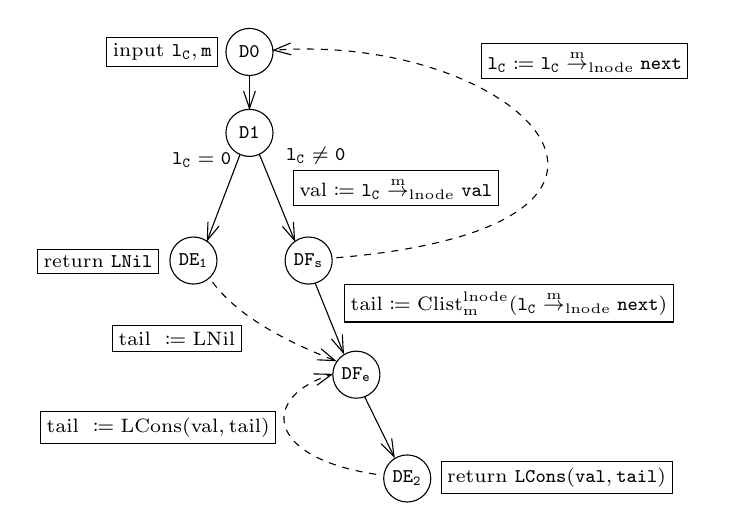
\begin{tikzpicture}[x=0.75pt,y=0.75pt,yscale=-1,xscale=1]
%uncomment if require: \path (0,558); %set diagram left start at 0, and has height of 558

% Text Node
\draw    (152, 55.5) circle [x radius= 11.34, y radius= 11.34]   ;
\draw (152,55.5) node  [font=\scriptsize]  {\tt D0};
% Text Node
\draw    (152, 94.5) circle [x radius= 11.34, y radius= 11.34]   ;
\draw (152,94.5) node  [font=\scriptsize]  {\tt D1};
% Text Node
\draw    (125, 156) circle [x radius= 11.34, y radius= 11.34]   ;
\draw (125,156) node  [font=\scriptsize]  {\tt DE$\mathrm{\tt _1}$};
% Text Node
\draw    (180.5, 156) circle [x radius= 11.34, y radius= 11.34]   ;
\draw (180.5,156) node  [font=\scriptsize]  {\tt DF$\mathrm{\tt _s}$};
% Text Node
\draw    (203.5, 211) circle [x radius= 11.34, y radius= 11.34]   ;
\draw (203.5,211) node  [font=\scriptsize]  {\tt DF$\mathrm{\tt _e}$};
% Text Node
\draw    (228, 261) circle [x radius= 11.34, y radius= 11.34]   ;
\draw (228,261) node  [font=\scriptsize]  {\tt DE$\mathrm{\tt _2}$};
% Text Node
\draw (129,107.5) node  [font=\scriptsize]  {${\tt l_{C}=0}$};
% Text Node
\draw (184,105.5) node  [font=\scriptsize]  {${\tt l_{C}\neq 0}$};
% Text Node
\draw (79,156.5) node  [font=\scriptsize]  {\setlength{\fboxsep}{2pt}\fbox{$\mathrm{return\ \tt LNil}$}};
% Text Node
\draw (222.5,121) node  [font=\scriptsize]  {\setlength{\fboxsep}{2pt}\fbox{$\mathrm{val \coloneqq \structPointer{l_{C}}{m}{lnode}{val}}$}};
% Text Node
\draw (277,176.5) node  [font=\scriptsize]  {\setlength{\fboxsep}{2pt}\fbox{$\mathrm{tail \coloneqq Clist_{m}^{lnode}(\structPointer{l_{C}}{m}{lnode}{next})}$}};
% Text Node
\draw (300,260.5) node  [font=\scriptsize]  {\setlength{\fboxsep}{2pt}\fbox{$\mathrm{return\ \tt LCons( val,tail)}$}};
% Text Node
\draw (313.5,60) node  [font=\scriptsize]  {\setlength{\fboxsep}{2pt}\fbox{$\mathrm{{\tt l_{C}} \coloneqq \structPointer{l_{C}}{m}{lnode}{next}}$}};
% Text Node
\draw (117,193.5) node  [font=\scriptsize]  {\setlength{\fboxsep}{2pt}\fbox{$\mathrm{tail\ \coloneqq LNil}$}};
% Text Node
\draw (108,236.5) node  [font=\scriptsize]  {\setlength{\fboxsep}{2pt}\fbox{$\mathrm{tail\ \coloneqq LCons( val,tail)}$}};
% Text Node
\draw (110,55.5) node  [font=\scriptsize]  {\setlength{\fboxsep}{2pt}\fbox{$\mathrm{input\ \tt l_{C},m}$}};
% Connection
\draw  [-{Straight Barb[length=2.2mm, width=1.5mm]}]  (152,66.6) -- (152,83.5) ;
% Connection
\draw  [-{Straight Barb[length=2.2mm, width=1.5mm]}]  (147.54,104.67) -- (131.39,147) ;
% Connection
\draw  [-{Straight Barb[length=2.2mm, width=1.5mm]}]  (156.67,104.58) -- (174,147) ;
% Connection
\draw  [-{Straight Barb[length=2.2mm, width=1.5mm]}]  (183.7,167) -- (197.53,201.2) ;
% Connection
\draw  [-{Straight Barb[length=2.2mm, width=1.5mm]}]  (207.43,221.5) -- (222.01,251.2) ;
% Connection
\draw  [-{Straight Barb[length=2.2mm, width=1.5mm]},dash pattern={on 2.5pt off 2.5pt}]  (134.22,166.39) .. controls (143.79,179.47) and (162.27,192.18) .. (194,204.5) ;
% Connection
\draw  [-{Straight Barb[length=2.2mm, width=1.5mm]},dash pattern={on 2.5pt off 2.5pt}]  (193.9,154.67) .. controls (375.75,139.13) and (281.42,46.11) .. (162.84,54.72) ;
%Curve Lines [id:da3594688465785896] 
\draw  [-{Straight Barb[length=2.2mm, width=1.5mm]},dash pattern={on 2.5pt off 2.5pt}]  (213,259) .. controls (159.61,251.02) and (156.87,221.8) .. (192.44,210.59) ;

\end{tikzpicture}

% % Text Node
% \draw    (152, 55.5) circle [x radius= 11.34, y radius= 11.34]   ;
% \draw (152,55.5) node  [font=\scriptsize]  {\tt D0};
% % Text Node
% \draw    (152, 106.5) circle [x radius= 11.34, y radius= 11.34]   ;
% \draw (152,106.5) node  [font=\scriptsize]  {\tt D1};
% % Text Node
% \draw    (121, 176) circle [x radius= 11.34, y radius= 11.34]   ;
% \draw (121,176) node  [font=\scriptsize]  {\tt DE$\mathrm{_1}$};
% % Text Node
% \draw    (180.5, 175) circle [x radius= 11.34, y radius= 11.34]   ;
% \draw (180.5,175) node  [font=\scriptsize]  {\tt DF$\mathrm{_s}$};
% % Text Node
% \draw    (205.5, 237) circle [x radius= 11.34, y radius= 11.34]   ;
% \draw (205.5,237) node  [font=\scriptsize]  {\tt DF$\mathrm{_e}$};
% % Text Node
% \draw    (231, 296) circle [x radius= 11.34, y radius= 11.34]   ;
% \draw (231,296) node  [font=\scriptsize]  {\tt DE$\mathrm{_2}$};
% % Text Node
% \draw (127,120.5) node  [font=\scriptsize]  {${\tt l_{C}=0}$};
% % Text Node
% \draw (190,119.5) node  [font=\scriptsize]  {${\tt l_{C}\neq 0}$};
% % Text Node
% \draw (74,175.5) node  [font=\scriptsize]  {\setlength{\fboxsep}{2pt}\fbox{$\mathrm{return\ \tt LNil}$}};
% % Text Node
% \draw (225.5,137) node  [font=\scriptsize]  {\setlength{\fboxsep}{2pt}\fbox{$\mathrm{val \coloneqq \structPointer{l_{C}}{m}{lnode}{val}}$}};
% % Text Node
% \draw (284.5,199.5) node  [font=\scriptsize]  {\setlength{\fboxsep}{2pt}\fbox{$\mathrm{tail \coloneqq Clist_{m}^{lnode}(\structPointer{l_{C}}{m}{lnode}{next})}$}};
% % Text Node
% \draw (305,296) node  [font=\scriptsize]  {\setlength{\fboxsep}{2pt}\fbox{$\mathrm{return\ \tt LCons( val,tail)}$}};
% % Text Node
% \draw (332.5,80) node  [font=\scriptsize]  {\setlength{\fboxsep}{2pt}\fbox{$\mathrm{{\tt l_{C}} \coloneqq \structPointer{l_{C}}{m}{lnode}{next}}$}};
% % Text Node
% \draw (90,213.5) node  [font=\scriptsize]  {\setlength{\fboxsep}{2pt}\fbox{$\mathrm{tail\ \coloneqq LNil}$}};
% % Text Node
% \draw (95,275.5) node  [font=\scriptsize]  {\setlength{\fboxsep}{2pt}\fbox{$\mathrm{tail\ \coloneqq LCons( val,tail)}$}};
% % Text Node
% \draw (108,54.5) node  [font=\scriptsize]  {\setlength{\fboxsep}{2pt}\fbox{$\mathrm{input\ \tt l_{C},m}$}};
% % Connection
% \draw [-{Straight Barb[length=2.2mm, width=1.5mm]}]    (152,66.6) -- (152,95.5) ;
% % Connection
% \draw [-{Straight Barb[length=2.2mm, width=1.5mm]}]    (147.48,116.6) -- (125.5,166) ;
% % Connection
% \draw [-{Straight Barb[length=2.2mm, width=1.5mm]}]    (156.27,116.6) -- (174,166) ;
% % Connection
% \draw [-{Straight Barb[length=2.2mm, width=1.5mm]}]    (184,186) -- (200,227) ;
% % Connection
% \draw [-{Straight Barb[length=2.2mm, width=1.5mm]}]    (209,248) -- (226,286) ;
% % Connection
% \draw  [-{Straight Barb[length=2.2mm, width=1.5mm]},dash pattern={on 2.5pt off 2.5pt}]  (121.12,187.73) .. controls (124.23,219.54) and (146.76,235.03) .. (194.8,234.5) ;
% % Connection
% \draw  [-{Straight Barb[length=2.2mm, width=1.5mm]},dash pattern={on 2.5pt off 2.5pt}]  (191.95,174.53) .. controls (378.87,170.91) and (282.78,56.07) .. (162.88,55.73) ;
% %Curve Lines [id:da3594688465785896] 
% \draw  [-{Straight Barb[length=2.2mm, width=1.5mm]},dash pattern={on 2.5pt off 2.5pt}]  (219,297) .. controls (154.43,294.92) and (142.05,247.86) .. (197,244) ;

% \end{tikzpicture}

\end{document}
